\documentclass[spanish]{textolivre}

% metadata
\journalname{Texto Livre}
\thevolume{17}
%\thenumber{1} % old template
\theyear{2024}
\receiveddate{\DTMdisplaydate{2024}{3}{20}{-1}}
\accepteddate{\DTMdisplaydate{2024}{7}{2}{-1}}
\publisheddate{\today}
\corrauthor{Noelia Estévez Rionegro}
\articledoi{10.1590/1983-3652.2024.51696}
%\articleid{NNNN} % if the article ID is not the last 5 numbers of its DOI, provide it using \articleid{} commmand 
% list of available sesscions in the journal: articles, dossier, reports, essays, reviews, interviews, editorial
\articlesessionname{articles}
\runningauthor{Estévez Rionegro y Cea Álvarez}
%\editorname{Leonardo Araújo} % old template
\sectioneditorname{Hugo Heredia Ponce}
\layouteditorname{João Mesquita}

\title{Optimización tecnológica en el entrenamiento estratégico para mejorar la competencia ortográfica: percepción de los aprendices de español L2 con L1 portugués}
\othertitle{Otimização tecnológica na formação estratégica para melhorar a competência ortográfica: percepção de alunos de espanhol L2 com português L1}
\othertitle{Technological enhancement in strategic training to improve spelling competence: perception of Spanish L2 learners with Portuguese L1}

\author[1]{Noelia Estévez-Rionegro~\orcid{0000-0002-7828-5339}\thanks{Email: \href{mailto:noelia.rionegro@usc.es}{noelia.rionegro@usc.es}}}
\author[2]{Ana María Cea Álvarez~\orcid{0000-0002-7383-9646}\thanks{Email: \href{mailto:anacea@elach.uminho.pt}{anacea@elach.uminho.pt}}}
\affil[1]{Universidade de Santiago de Compostela, Facultad de Formación del Profesorado, Departamento de Didácticas Aplicadas, Lugo, Galicia, España.}
\affil[2]{Universidade do Minho, Escola de Letras, Artes e Ciências Humanas, Departamento de Estudos Românicos, Campus de Gualtar, Braga, Portugal.}

\addbibresource{article.bib}

\usepackage[inline]{enumitem}
\usepackage{array}

\begin{document}
\maketitle
\begin{polyabstract}
\begin{abstract}
Esta contribución se centra en el análisis de la percepción de los aprendices de español como L2 con L1 portugués sobre su competencia ortográfica en L2 antes y después de realizar un entrenamiento con la integración de diferentes recursos relacionados con las Tecnologías de la Información y la Comunicación (TIC). Este entrenamiento ha sido ideado a partir de un diagnóstico de errores comunes identificados en estudios precedentes. De los resultados obtenidos en las encuestas realizadas en \textit{Google Forms}, elaboradas \textit{ad hoc} para la recogida de datos, se extrae que el grupo meta es consciente de sus dificultades ortográficas derivadas de interferencias y/o transferencias lingüísticas por proximidad etimológica entre la L1 y la L2 (aunque en algunos casos esas características supongan una ventaja en su nivel general de español), corroborando el diagnóstico de la literatura científica. Mayoritariamente, los informantes consideran que el entrenamiento con recurso a aplicaciones digitales (como el \textit{software Read \& Write} de \textit{Google Chrome} que mejora la ortografía con la predicción de palabras a través del reconocimiento de texto y otras funciones) ha contribuido a promover la competencia ortográfica y a que los estudiantes perciban efectividad en el diseño, organización y recursos del entrenamiento.

\keywords{Ortografía \sep Español L2 \sep Autopercepción \sep Sistema de entrenamiento TIC}
\end{abstract}

\begin{portuguese}
\begin{abstract}
Esta contribuição centra-se na análise da percepção dos aprendizes de espanhol como L2 com português L1 sobre a sua competência ortográfica em L2 antes e depois de uma formação com a integração de diferentes recursos relacionados com as Tecnologias de Informação e Comunicação (TIC). Este treinamento foi concebido a partir de um diagnóstico de erros comuns identificados em estudos anteriores. A partir dos resultados obtidos nas entrevistas realizadas no \textit{Google Forms}, desenvolvidos \textit{ad hoc} para a recolha de dados, verifica-se que o grupo-alvo está consciente das suas dificuldades ortográficas decorrentes de interferências e/ou transferências linguísticas devido à proximidade etimológica entre a L1 e a L2 (embora em alguns casos essas características representem uma vantagem no seu nível geral de espanhol), corroborando o diagnóstico feito na literatura científica. A maioria dos informantes considera que a formação com recurso a aplicações digitais (como o \textit{software} \textit{Read \& Write} do \textit{Google Chrome}, que melhora a ortografia através da previsão de palavras por reconhecimento de texto e outras funções), contribuiu para a promoção da competência ortográfica e para a percepção dos alunos sobre a eficácia da concepção, organização e recursos do treinamento.

\keywords{Ortografia \sep Espanhol L2 \sep Autopercepção \sep Sistema de treinamento TIC}
\end{abstract}
\end{portuguese}

\begin{english}
\begin{abstract}
This paper focuses on the analysis of the perception of learners of Spanish as L2 with Portuguese L1 on their orthographic competence in L2 before and after a training with the integration of different resources related to Information and Communication Technologies (ICT). This training has been devised on the basis of a diagnosis of common errors identified in previous studies. From the results obtained in the surveys carried out in Google Forms, developed \textit{ad hoc} for data collection, it can be seen that the target group is aware of their spelling difficulties arising from interference and/or linguistic transfers due to etymological proximity between L1 and L2 (although in some cases these characteristics constitute an advantage in their general level of Spanish), which confirms the diagnosis made in the scientific literature. The vast majority of informants consider that training with the use of digital applications (such as Google Chrome's Read \& Write software, which improves spelling by predicting words through text recognition and other functions) has contributed to fostering spelling competence and to students' perception of the effectiveness of the design, organisation and resources of the training.

\keywords{Spelling \sep Spanish L2 \sep Awareness \sep ICT training system}
\end{abstract}
\end{english}
\end{polyabstract}

\section{Introducción}
El dominio de la ortografía constituye uno de los aspectos básicos en la adquisición de una lengua. Las dificultades específicas que experimentan, concretamente, los falsos principiantes (estudiantes que no parten de cero y poseen algunos conocimientos del sistema lingüístico y pragmático de la lengua que aprenden) y los aprendientes de alta velocidad de aprendizaje, producto de la proximidad etimológica entre su L1 y la lengua meta \cite{centro_virtual_cervantes_falso_2008} (s.v. “falso principiante”), urgen la detección e identificación temprana de los errores en los aprendices, a fin de reconducir su aprendizaje, reforzarlo en los puntos oportunos y evitar su fosilización en la interlengua. Para ello, cabe tener en cuenta no solo el diagnóstico de errores que pueda realizarse, ya sea a partir de un análisis empírico o de la literatura científica publicada, sino también la percepción de los aprendices sobre la progresión de su propia competencia ortográfica.

En este trabajo, hemos llevado a cabo un análisis de los estudios precedentes, que permitió obtener un prediagnóstico de errores comunes en los aprendices de ELE con L1 portugués, sobre el que sentar las bases para el diseño de un sistema de entrenamiento con recurso a las TIC (sustentado en la eficacia de determinados recursos tecnológicos en experiencias previas) que contribuyese a reforzar los aspectos ortográficos más dificultosos en este perfil de estudiantes. Para determinar su eficacia, se puso en práctica con un grupo de participantes, cuya percepción en torno a su propia competencia ortográfica se indagó antes y después de la intervención mediante encuestas con preguntas cerradas elaboradas \textit{ad hoc} para esta investigación. El análisis de los datos obtenidos permitió conocer (i) el grado de consciencia de los falsos principiantes en ELE sobre sus errores ortográficos comunes y sus conocimientos sobre recursos tecnológicos que contribuyen al desarrollo de esta competencia, (ii) su percepción sobre su propia progresión en el proceso de adquisición de la ortografía mediante el sistema de entrenamiento TIC diseñado y (iii) su valoración sobre la efectividad de ese sistema como recurso didáctico y como herramienta tecnológica.   

\section{Marco teórico}\label{sec-normas}
La competencia ortográfica, de acuerdo con el \textit{Marco Común Europeo de Referencia para las Lenguas} (MCERL) \cite[p. 114]{consejo_de_europa_marco_2001} “supone el conocimiento y la destreza en la percepción y la producción de los símbolos de que se componen los textos escritos”. En las lenguas alfabéticas, como el español, un aprendiz debe ser capaz de percibir y de producir la forma de las letras, la correcta ortografía de las palabras, los signos de puntuación, las convenciones tipográficas y los signos no alfabetizables de uso común \cite{consejo_de_europa_marco_2001}. Está estrechamente relacionada con la competencia ortoépica, pues el dominio de la pronunciación, a partir de la forma escrita, implica el conocimiento de las convenciones ortográficas \cite{consejo_de_europa_marco_2001}. Aspectos como la articulación, la pronunciación o la asociación entre sonidos y grafías están directamente involucrados en la adquisición de la competencia ortográfica, aunque esta siempre tenga como soporte la escritura. Su dominio se determina, por tanto, en la evaluación de la expresión escrita, a partir de los parámetros y distribución por niveles que establece el MCERL (\textit{vid.} \textcite{consejo_de_europa_marco_2001}). Para lograr el desarrollo de la capacidad de control del sistema de escritura, se sugiere la realización de diversas prácticas: escritura a mano, dictado, exposición a textos auténticos y diversos, etc. \cite{consejo_de_europa_marco_2001}.

Por su parte, el \textit{Plan Curricular} del \textcite{instituto_cervantes_plan_2006} dedica su cuarto bloque a los aspectos ortográficos, con un inventario para todos los niveles de lengua cuya finalidad es “adecuar su presentación y su nivelación a las necesidades comunicativas del alumno, al desarrollo de su proceso de aprendizaje y a la relación entre los elementos ortográficos y los otros niveles de estructuración lingüística” \cite{instituto_cervantes_plan_2006}. Así, se distribuyen entre los niveles A1 y C2 los diferentes contenidos sobre cada uno de los siguientes aspectos generales: 
\begin{enumerate*}[label=(\roman*)]
\item ortografía de letras y palabras, 
\item acentuación gráfica, 
\item puntuación y 
\item abreviaturas y siglas. 
\end{enumerate*}
Competen directamente a este estudio los dos primeros, centrados en las relaciones entre el sistema grafemático y el fonológico, la ortografía léxica y el sistema acentual. Dada su importancia como base de la competencia ortográfica, su correcta asimilación en los primeros niveles debe ser uno de los principales objetivos para el desarrollo de la expresión escrita en el proceso de adquisición de una L2. En un plano más amplio, la competencia comunicativa está relacionada con la habilidad para (des)codificar la lengua meta (comprender el significado y usar las formas adecuadamente). En consecuencia, el dominio de la gramática (en el que se incluyen las dimensiones antes mencionadas: ortográfica y ortoépica) permitirá alcanzar un nivel de comunicación más elevado, tanto en una L1 como en L2. Además, el hecho de conocer las dificultades del alumnado desde los niveles iniciales, que capacitan al aprendiz como “usuario básico” de la lengua y sientan las bases lingüísticas que le permitirán afrontar con solvencia una formación intermedia \cite{consejo_de_europa_marco_2001}, permite corregir tempranamente sus errores y evitar que fosilicen.

Asimismo, para lograr este objetivo, es necesario tener en cuenta la lengua inicial de los aprendices, ya que puede influir en el proceso de adquisición de la L2. Como se mostrará en el apartado siguiente, la proximidad lingüística entre el español y el portugués convierte a este perfil de aprendices en “falsos principiantes”, porque poseen ciertos conocimientos lingüísticos y pragmáticos de español, pero estos no son suficientes para ubicarlos en un nivel superior \cite{alvite_importancia_2004}. Sin embargo, como muestra la literatura científica, esta aparente ventaja se ve contrarrestada por la frecuente presencia de errores provocados, entre otros, por interferencia lingüística, de modo que este perfil de alumnado presenta mayor facilidad para la comprensión lectora \cite{Soares_2019}, pero tiene más dificultades en la práctica oral, al no distinguir las diferencias fónicas entre los sistemas lingüísticos de los dos idiomas \cite{buchener_alise_2019,ribeiro_enfoque_2021}.

\subsection{La competencia ortográfica de los aprendices con L1 portugués}\label{sec-conduta}
El español y el portugués son, de las lenguas románicas, las que más se parecen en todos los niveles \cite{almeida_uma_1995}. Esta proximidad supone una ventaja para los aprendices, en tanto que la semejanza que perciben entre las dos lenguas los lleva a afrontar el aprendizaje con mayor confianza y a avanzar más rápido en los primeros niveles que los hablantes de otras lenguas \cite{capilla_o_2009}. Sin embargo, en los niveles siguientes, se produce un retroceso y un estancamiento en el progreso de la interlengua, producto de una pérdida de motivación comunicativa y de la aparición de dificultades derivadas de interferencias lingüísticas, que se manifiestan en la presencia de errores fosilizados \cite[p. 2]{capilla_o_2009} y que \textcite{dominguez_vazquez_en_2001} interpreta como un proceso de automatización (selección automática de un elemento del código lingüístico de la L1 y su empleo inconsciente en la L2). En niveles superiores, contrariamente, los aprendices suelen haber tomado conciencia de los problemas comunicativos que causan las divergencias entre las dos lenguas y terminan por dominar las reglas de cada una \cite{torijano_errores_2004}.

Los estudios que analizan los errores ortográficos de los aprendices de español con L1 portugués coinciden al identificar los fallos más comunes derivados de las interferencias por proximidad lingüística en diferentes perfiles de alumnado. \textcite[p. 30]{perez_ensenanza_2007} señala como errores frecuentes de los estudiantes portugueses recién ingresados en la universidad (con base previa de español adquirida durante la educación secundaria) los de acentuación (por omisión, como *\textit{aqui}, o por adición, como *\textit{armário}), cambio de grafías (*\textit{escuro}) y duplicación de la “s” (*\textit{necessario}). \textcite{andrade_neta_aprender_2000}, por su parte, detecta errores de acentuación relativos al timbre, el acento grave y circunflejo, la tilde y la marca de nasalización, junto a las dificultades con la “ç” y los dígrafos “ss”, “lh”, “nh” y “rr” en los estudiantes brasileños. \textcite{baerlocher_rocha_errores_2013} detecta, en léxico del profesorado de ELE en formación, la presencia de errores por adición u omisión de acentos; por adición, omisión o sustitución de letras; por confusión de grafías motivada etimológicamente (fonema /b/, grafías “v” y “b”; fonema /s/, grafías “ss” y “s”; fonema /k/, grafías “qu” y “c”; fonema /x/, grafías “j” y “g”), y otros de diptongación. La autora llama la atención sobre el hecho de que, en los niveles avanzados, los aprendices todavía tienen algunas dificultades para establecer los límites entre las dos lenguas, aunque estas se hayan reducido considerablemente con respecto a niveles inferiores \cite{baerlocher_rocha_errores_2013}. Por último, \textcite{cardoso_interferencias_2022} encuentran dificultades en los aprendices adultos de nivel intermedio y avanzado en el empleo de grafemas que representan sonidos próximos en vocablos con grafías similares en las dos lenguas (“v-b”, “q-c”, “d-t”, “i-e”, “f-h” y “m-n” al final de una palabra) y del dígrafo “ss”. Los autores sitúan en un 94~\% el porcentaje de errores por influencia de la lengua portuguesa detectados en su análisis y los relacionan con la confusión en la asociación entre sonidos y grafías; razón por la cual, como se sostenía en la introducción del apartado, la relación entre la competencia ortográfica y la competencia ortoépica debería constituir uno de los focos de atención en la enseñanza y aprendizaje de lenguas extranjeras, especialmente si estas son etimológicamente próximas a la materna.

No obstante, aun siendo las interferencias de la L1 en la L2 la principal fuente de errores en el aprendizaje de lenguas próximas \cite{capilla_o_2009}, no debemos tomar la semejanza etimológica como algo negativo, pues la transferencia lingüística, entendida como transmisión de un conocimiento previo correctamente aplicado \cite{brown_principles_2000}, puede facilitar el aprendizaje de la L2. Así lo perciben, de hecho, los propios aprendices, que ven más ventajas que inconvenientes en el contacto lingüístico entre su L1 y la lengua meta \cite{aires_influencia_2018,espinosa_creencias_2009}.


\subsection{Las tecnologías en el desarrollo de la competencia ortográfica}\label{sec-fmt-manuscrito}
El continuo avance de las TIC ha tenido una importante repercusión en los procesos de enseñanza-aprendizaje y el aprovechamiento de su potencial educativo es uno de los principales retos para el docente del siglo XXI \cite{unesco_competencias_2016}. El Instituto Nacional de Tecnologías y de Formación del Profesorado (INTEF) destaca la importancia de la competencia digital, concebida como el uso crítico y seguro de las TIC para alcanzar los objetivos relacionados con el aprendizaje, la inclusión y la participación en la sociedad actual \cite{instituto_nacional_de_tecnologias_y_de_formacion_del_profesorado_instituto_2017}. Diferentes autores han tratado de definir las prácticas educativas que emplean las TIC de forma eficaz \cite{budhwar_role_2017,Scaradozzi_2019,Blikstein_2021} y destacar sus beneficios en el rendimiento de los estudiantes, el fomento de su creatividad y el desarrollo de su capacidad para la resolución de problemas \cite{odorico_marco_2004,marques_graells_impacto_2013}. Se trata de prácticas innovadoras y motivacionales que facilitan el proceso de enseñanza y aprendizaje y favorecen la alfabetización digital del alumnado \cite{budhwar_role_2017}. En definitiva, las TIC son capaces de modificar significativamente la forma de enseñar y la manera de aprender \cite{odorico_marco_2004}.

La verdadera importancia de las TIC en la educación radica en su empleo como un medio de enseñanza que permita conseguir objetivos educativos concretos \cite{blazquez_propuesta_2018}. Con esta idea, surgen las Tecnologías del Aprendizaje y el Conocimiento (TAC), una orientación formativa de las TIC que apuesta por un enfoque más pedagógico que permita explorar el uso de las herramientas tecnológicas para la adquisición de conocimiento \cite{lozano_tic_2011}; no se trata de integrar las TIC en el aula, sino de intentar convertirlas en un recurso para el aprendizaje (2008). Uno de sus principales valores estriba en que permiten acceder a un gran conjunto de herramientas digitales para diseñar materiales didácticos \cite{garcia_tecnologias_2020}, como editores de vídeo, plataformas de gamificación y herramientas para la creación de contenidos (\textit{vid.} \textcite{pimbo_tiban_tecnologias_2022}.

El aprovechamiento de su potencial para la enseñanza específica de lenguas puede concretarse en la creación de materiales o en la práctica de contenidos mediante aplicaciones y recursos especializados en la modalidad oral o escrita \cite{vazquez-cano_nuevas_2014,estevez_rionegro_tecnologias_2024}, aunque también pueden integrar las dos para trabajarlas de manera simultánea. Es el caso de los documentos de \textit{Google Chrome} implementados con el \textit{plug-in Read\&Write}, que ofrecen un conjunto de herramientas adicionales con las que contribuir al aprendizaje simultáneo de la lecto-escritura y cuyos beneficios en los estudiantes son destacados por autores como \textcite{liou_training_2009,pim_emerging_2013} o el \textcite{departamento_de_educacion_de_la_comunidad_autonoma_del_pais_vasco_propuestas_2020}. Este software cuenta con funciones como la conversión de texto a voz, la predicción de palabras, los diccionarios integrados y el resaltado de texto. Todo ello proporciona ayuda instantánea a los alumnos y esto se ha relacionado con mejoras en las destrezas implicadas, ofreciendo, a su vez, una experiencia de escritura no solo más agradable, sino formalmente más correcta \cite{orr_assisted_2007,ok_digital_2019}. Estas funciones resultan especialmente interesantes para afianzar la relación entre sonidos y grafías en ELE, al trabajar, de manera simultánea, varias destrezas en las que están implicadas las dos modalidades de la lengua: la pronunciación, a través de la lectura en voz alta, y la ortografía, mediante la trascripción de audiciones. En este sentido, \textit{Read\&Write} permitiría integrar los aspectos de ortografía y ortoépica sugeridos en la introducción del marco teórico.

Si bien existen otras aplicaciones de lectura y escritura asistida con funciones similares, como pueden ser \textit{Freedom Scientific’s WYNN o Kurzweil’s kurzweil 3000}, estas están pensadas para alumnado con necesidades educativas especiales que afectan a la ortografía, como la dislexia o la disgrafía \cite{orr_assisted_2007}, mientras que \textit{Read\&Write} es un software de refuerzo destinado a estudiantes sin dificultades específicas.

Otras TAC que resultan especialmente útiles en la enseñanza y aprendizaje de lenguas propias y extranjeras y que competen directamente a este estudio son aquellas que permiten la creación de murales virtuales dinámicos e interactivos, como el \textit{Padlet} \cite{servio_padlet:_2022,conceicao_as_2022}. Estas herramientas resultan especialmente provechosas para el desarrollo de competencias comunicativas orales y escritas (así lo han destacado \textcite{vazquez-cano_nuevas_2014,estevez_rionegro_tecnologias_2024}), y sus ventajas en la adquisición del español como L2 han sido probados en investigaciones precedentes \cite{stinga_fortaleciendo_2021,gonzalez_enfoque_2023}.


\section{Objetivos e hipótesis del estudio}\label{sec-formato}
El estudio que se describe pretendía: 
\begin{enumerate*}[label=(\roman*)]
\item conocer y comparar la percepción de los estudiantes meta sobre su competencia lingüística en la dimensión ortográfica antes y después del entrenamiento al que fueron sometidos; 
\item comprobar si el sistema de entrenamiento con recurso a las TIC, que integraba actividades de ortografía y ortoépica, resultaba eficaz para reforzar el desarrollo de falsos principiantes de español L2.
\end{enumerate*}
De acuerdo con lo anterior, en el momento inicial de la investigación se plantearon las siguientes hipótesis:

\begin{enumerate}[label=(\roman*)]
    \item Dada la proximidad etimológica y geográfica entre las lenguas española y portuguesa, los aprendices portugueses de español L2 experimentan cierta facilidad en adquirir las reglas ortográficas de la lengua meta, sobre todo en los primeros niveles de aprendizaje (A1 y A2). Sin embargo, manifiestan también algunas dificultades en la asociación de determinados sonidos con sus correspondientes grafías debido a las divergencias lingüísticas que existen entre ambas lenguas.
    \item El cuestionario de autopercepción sobre el entrenamiento para el desarrollo de la competencia ortográfica de los estudiantes ampliaría su conciencia sobre el proceso de aprendizaje, sobre la eficacia de los recursos TIC y, en consecuencia, contribuiría al desarrollo de su autonomía.
\end{enumerate}

\section{Metodología de investigación}\label{sec-modelo}
El foco principal de este estudio pretendía analizar en dos momentos diferentes la autopercepción de los estudiantes sobre su competencia ortográfica y estratégica en relación con su participación en un entrenamiento con recurso a las TIC.  Para la recogida de datos, se diseñó una encuesta que fue autoadministrada a través de un muro de \textit{Padlet}, el mismo que alojaba las actividades del sistema de entrenamiento (vid. \Cref{fig1}). Se trata de un modelo de investigación óptimo para este tipo de estudios, puesto que proporciona a los encuestados mayor sensación de privacidad que otros métodos (como las entrevistas), lo que favorece la calidad de sus respuestas \cite{cea_dancona_metodos_2004,fernandez-vazquez_muda_2023}.

\subsection{Diseño del estudio, contexto y participantes}\label{sec-organizacao}
El desarrollo de la competencia lingüística de los estudiantes fue acotado a la observación de la subcompetencia ortográfica y, en ese sentido, se diseñó un entrenamiento ortográfico y estratégico ad hoc que fue implementado en modalidad híbrida (presencial y a distancia) gracias a un soporte digital. La mencionada instrucción, que sirvió como \textit{input} y estímulo de la investigación, pretendía ofrecer una respuesta didáctica a algunas de las necesidades de aprendizaje descritas en la bibliografía \cite{andrade_neta_aprender_2000,perez_ensenanza_2007,baerlocher_rocha_errores_2013,cardoso_interferencias_2022} para el siguiente perfil del grupo meta: estudiantes de iniciación de español como L2 que presentan una serie de desviaciones de la norma en la dimensión ortográfica, producto, en su mayoría, de las dificultades encontradas en esta fase temprana de adquisición y que pueden estar relacionadas con interferencias de la L1 o dificultades de adquisición propias de L2.  

Así pues, la parte empírica de esta investigación se llevó a cabo en la Escola de Letras, Artes e Ciências Humanas de la Universidade do Minho, en el campus de Gualtar (Braga, Portugal) y los informantes que formaron parte del estudio estaban matriculados en una asignatura optativa del segundo curso denominada “Introdução à língua e cultura española”. Esta asignatura pertenece al grado de Línguas Aplicadas y se imparte en régimen de clases presenciales. En lo que concierne al contexto temporal y al número de alumnos totales que participó en el estudio, contamos con 21 alumnos durante el segundo semestre del curso 2022-2023. Aunque el reducido número de participantes no permite generalizar los resultados, las hipótesis han sido contrastadas en la literatura científica (las dificultades específicas que encuentran los falsos principiantes de portugués L1 que estudian español L2), y el estudio nos ha permitido analizar de forma intensiva la realidad acotada.

El perfil académico de los estudiantes era heterogéneo, pues una parte de ellos pertenecía a la Licenciatura de Línguas Aplicadas, mientras que el resto de los alumnos procedía de otras titulaciones y se matriculan en esta asignatura como materia de libre elección. Su perfil lingüístico, sin embargo, era semejante: se trataba de alumnos de portugués como L1 que poseían un nivel de iniciación en español como L2. Más concretamente, se trataba de un nivel de lengua equivalente al A2 del \textcite{consejo_de_europa_marco_2001}. Sin embargo, la proximidad geográfica y etimológica entre las dos lenguas (L1 y L2), como ya hemos avanzado, permite que el perfil general de este alumnado los considere como “falsos principiantes”.

Por último, debemos señalar que la confidencialidad de los datos de todos los participantes quedó garantizada mediante la firma de un consentimiento informado.

\subsection{Instrumentos de investigación}\label{sec-organizacao-latex}
A fin de analizar la autopercepción de los estudiantes sobre su evolución en la competencia ortográfica a lo largo del entrenamiento, se diseñaron dos cuestionarios que se implementaron en dos momentos diferentes (antes y después del entrenamiento estratégico) y cuyos datos fueron objeto de un tratamiento cuantitativo antes de proceder al análisis de resultados. Para lograr obtener respuestas más estandarizadas, los cuestionarios se elaboraron \textit{ad hoc} en \textit{Google Forms}, mediante preguntas cerradas medidas con la escala aditiva de Likert y con escala nominal.

Así pues, antes de comenzar el entrenamiento ortográfico, los estudiantes respondieron a una encuesta sobre sus hábitos ortográficos, compuesta por 15 preguntas cerradas sobre tres bloques temáticos. Este cuestionario pretendía corroborar 
\begin{enumerate*}[label=(\roman*)]
\item el inventario de variaciones de la norma ortográfica que los estudiantes, con este perfil lingüístico, serían susceptibles de producir en esta fase de su interlengua; 
\item identificar su nivel de competencia ortográfica en L2 antes de dar inicio al entrenamiento; e 
\item indagar sobre su conocimiento y manejo de herramientas TIC para subsanar esos mismos errores.
\end{enumerate*}

En la parte final del entrenamiento se aplicó otro cuestionario, que constaba igualmente de 15 preguntas cerradas y estaban organizadas en tres bloques. Este segundo cuestionario pretendía recoger información sobre la percepción de los participantes en relación con: 
\begin{enumerate*}[label=(\roman*)]
\item la eficacia del sistema de entrenamiento; 
\item la adecuación de las pruebas; y 
\item el funcionamiento de todo el proceso.
\end{enumerate*}

\subsection{Materiales y recursos empleados en el entrenamiento ortográfico}

El entrenamiento ortográfico se integró en la programación y evaluación general del curso, motivo por el cual los estudiantes realizaron a lo largo del entrenamiento, de un mes de duración, una serie de pruebas puntuables de carácter voluntario, consistentes en lecturas en voz alta automáticamente transcritas mediante un sistema de reconocimiento de voz y transcripciones de dictados orales en un documento de \textit{Google Chrome} con el \textit{plug-in Read\&Write}. Dado que el entrenamiento se implementó en modalidad híbrida y fue necesario recurrir a varias herramientas tecnológicas, uno de los pasos previos fue comprobar que los participantes disponían de los medios informáticos necesarios.

Las pruebas se fueron realizando tanto presencialmente en clase (sobre papel), como a distancia a través del \textit{Padlet}. Se trata de una herramienta en línea que permite crear un muro virtual dinámico e interactivo para grabar, guardar y compartir contenidos multimedia y en el cual se puede insertar cualquier tipo de contenido (texto, imágenes, vídeo, hipervínculos) \cite{conceicao_as_2022}. La utilización del muro virtual permitió desarrollar un trabajo ubicuo y colaborativo a lo largo del entrenamiento. Ese mismo soporte digital sirvió, también, para alojar, en archivos de texto en .pdf y archivos de audio en .mp3, los contenidos y actividades de los cuatro bloques temáticos que se pusieron en práctica (arte, turismo, gastronomía y música) y para disponibilizar las encuestas que debían responder los participantes (\Cref{fig1}).

\begin{figure}
    \centering
    \begin{minipage}{.85\textwidth}
    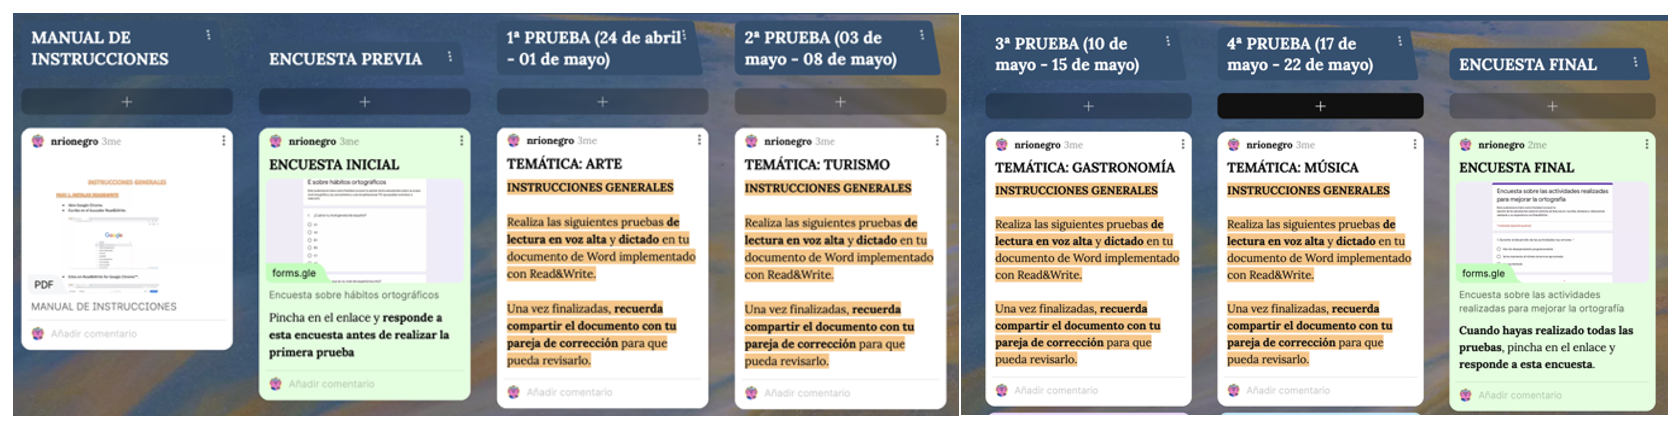
\includegraphics[width=\linewidth]{Fig1.png}
    \caption{Organización del entrenamiento estratégico en el muro virtual Padlet por bloques temáticos.}\label{fig1}
    \source{\url{https://es.padlet.com/nrionegro/sistema-de-pruebas-de-lectura-en-voz-alta-y-dictado-curso-20-lojoq4j8vd0cnsb6}}
    \end{minipage}
\end{figure}

Para responder a las actividades de entrenamiento disponibles en el \textit{Padlet}, se implementó un documento de \textit{Google Chrome} con la extensión \textit{Read\&Write}, que proporcionó apoyo a los procesos de lecto-escritura, puesto que el documento permite transcribir automáticamente los textos a través de un sistema de reconocimiento de voz. Este documento se utilizó para monitorizar la producción de textos y para permitir una evaluación colaborativa entre los estudiantes, que debían revisar, por parejas aleatorias, los textos resultantes (\textit{vid.} \Cref{fig2}).

\begin{figure}
    \centering
    \begin{minipage}{.85\textwidth}
    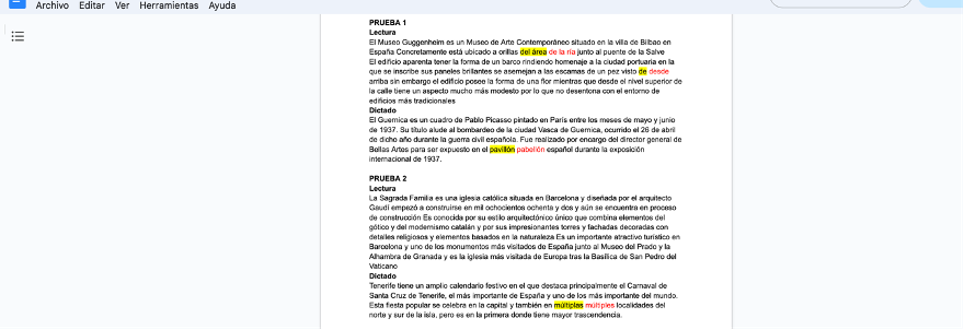
\includegraphics[width=\linewidth]{Fig2.png}
    \caption{Apariencia del documento final de las tareas realizadas por un participante.}\label{fig2}
    \source{\url{https://docs.google.com/}}
    \end{minipage}
\end{figure}

\section{Resultados y discusión}\label{sec-idioma}
En la \textit{Encuesta sobre hábitos ortográficos en español}, realizada antes de comenzar el sistema de entrenamiento, se parte de la percepción de los encuestados sobre su nivel general de español. Como se puede visualizar en la \Cref{tb1}, el 40,7~\% (esto es, la mayoría) apunta a un nivel B1; el 33,3~\% dice situarse en el A1; un 14,8~\%, en el A2; y el 11,1~\%, en el B2. Sobre su nivel en español en la destreza escrita, sin embargo, la mayoría (44,4~\%) se adscribe al nivel A1; el 25,9~\%, al A2; otro 25,9~\%, al B1; y solo la minoría restante (4,8~\%) dice situarse en el B2.

\begin{table}[htbp]
\centering
\begin{threeparttable}
\caption{Percepción del nivel de español general y escrito.}
\label{tb1}
\begin{tabular}{lllll}
\toprule
& A1 & A2 & B1 & B2 \\ 
\midrule
Nivel general & 33,30~\% & 14,80~\% & 40,70~\% & 11,10~\% \\
Nivel escrito & 44,40~\% & 25,90~\% & 25,90~\% & 4,80~\% \\
\bottomrule
\end{tabular}
\source{Elaboración propia.}
\end{threeparttable}
\end{table}

Esto supone que los participantes son conscientes de que su nivel de español baja cuando se evalúa únicamente la expresión escrita, donde los aprendices con L1 portugués tienen mayor dificultad; mientras que la proximidad entre las dos lenguas facilitaría otras destrezas, como la comprensión oral y escrita, que les haría sentirse en un nivel general de español superior. Esta idea permite matizar las sostenidas por autores como \textcite{brown_principles_2000,capilla_o_2009,espinosa_creencias_2009,aires_influencia_2018} sobre las ventajas e inconvenientes de la proximidad lingüística entre la L1 y la lengua meta, pues nuestros informantes reflejarían, en sus respuestas, una dificultad manifiesta en la expresión escrita y una facilidad percibida en las demás destrezas que, en su conjunto, los llevaría a sentirse en un nivel intermedio de español, a pesar de estar en el inicial. La percepción de los encuestados, en este punto, encaja perfectamente con el perfil del “falso principiante” \cite{alvite_importancia_2004,Soares_2019,budhwar_role_2017,ribeiro_enfoque_2021} descrito en el marco teórico, y refleja, además, que nuestros informantes serían conscientes de qué conocimientos lingüísticos y pragmáticos de español poseen para sentir que no parten de cero en su aprendizaje y de cuáles carecen para no poder situarse en un nivel superior.

En las siguientes preguntas del cuestionario, reconocen que, en general, suelen tener errores ortográficos en sus redacciones escritas: el 25,9~\% manifiesta tenerlos siempre; el 33,3~\%, frecuentemente; y el 40,7~\%, a veces. Ningún encuestado afirma no tenerlos nunca (\textit{vid.} \Cref{tb2}).

\begin{table}[htbp]
\centering
\begin{threeparttable}
\caption{Percepción general sobre la frecuencia de errores ortográficos.}
\label{tb2}
\begin{tabular}{lllll}
\toprule
& Siempre & Frecuentemente & A veces & Nunca  \\ 
\midrule
Errores ortográficos & 25,90~\% & 33,30~\% & 40,70~\% & 0,00~\% \\
\bottomrule
\end{tabular}
\source{Elaboración propia.}
\end{threeparttable}
\end{table}

De forma más específica, tratamos de ahondar en los errores que la literatura científica señala como comunes en los aprendices de español con L1 portugués, y que derivan de la proximidad etimológica entre las dos lenguas (\textit{vid.} \Cref{tb3}). Así, interrogados sobre esa tipología de errores en particular, solo un 3,9~\% manifiesta no tener dudas sobre la acentuación, pero el 15,4~\% las tiene siempre; un 26,9~\%, frecuentemente; y un 53,8~\%, a veces. Concretamente, las reglas de acentuación que son divergentes con respecto al portugués le generan dudas a un 51,9~\% a veces, a un 33,3~\% frecuentemente, y al 7,4~\% siempre; mientras que otro 7,4~\% manifiesta que no le ofrecen duda nunca.

En el caso de grafías que generalmente ofrecen confusión, los encuestados manifiestan lo siguiente: respecto a la doble “s”, el 25,9~\% no tiene dificultad nunca, mientras que el 55,6~\% la tiene a veces, el 11,1~\% la tiene frecuentemente y el 7,4~\% la tiene siempre; con la “ç”, la “nh” y la “lh” no tiene ninguna dificultad el 53,8~\%, pero sí la tiene siempre el 7,7~\%, frecuentemente el 23,1~\% y a veces el 15,4~\%; el 29,6~\% nunca duda entre escribir “s” o “c”, mientras que el 14,8~\% duda siempre, el 25,9~\% duda frecuentemente y el 29,6~\% solo a veces. Finalmente, entre la “c” y la “z” nunca duda el 25,9~\% y siempre duda el 14,8~\%, mientras que el 29,6~\% duda a veces y el 29,6~\% lo hace frecuentemente (\Cref{tb3}).  

\begin{table}[htbp]
\centering
\begin{threeparttable}
\caption{Percepción sobre la frecuencia de errores comunes por divergencia lingüística.}
\label{tb3}
\begin{tabular}{>{\raggedright}p{5.0cm} l l l l}
\toprule
& Siempre & \multicolumn{1}{>{\raggedright}p{1.5cm}}{Frecuen\-temente} & A veces & Nunca  \\ 
\midrule
Errores de acentuación & 7,40~\% & 33,30~\% & 51,90~\% & 7,40~\% \\
Dificultad con la doble “s” & 7,40~\% & 11,10~\% & 55,60~\% & 25,90~\% \\
Dificultad con “ç”, “nh” y “lh” & 7,70~\% & 23,10~\% & 15,40~\% & 53,80~\% \\
Confusión entre “s” y “c” & 14,80~\% & 25,90~\% & 29,60~\% & 29,60~\% \\
Confusión entre “c” y “z” & 14,80~\% & 29,60~\% & 29,60~\% & 25,90~\% \\
\bottomrule
\end{tabular}
\source{Elaboración propia.}
\end{threeparttable}
\end{table}

Observamos que, en general, la mayoría de los participantes son conscientes de los errores que cometen, y que son coincidentes con los señalados por \textcite{andrade_neta_aprender_2000,perez_ensenanza_2007,baerlocher_rocha_errores_2013,cardoso_interferencias_2022} que se recogen en el marco teórico. Sin embargo, cabe detenerse en el hecho de que un número bastante significativo de los encuestados manifiesta, como muestra la \Cref{tb3}, no tener dificultades en ninguno de los casos comunes señalados. Estos datos resultan aparentemente discordantes con respecto a los recogidos en la \Cref{tb2}, donde se refleja que ningún encuestado respondía negativamente al ser preguntado por la presencia de errores ortográficos en sus redacciones escritas. Cabría pensar \textit{a priori} que los errores que los encuestados perciben que cometen son diferentes a los señalados, pero solo con reservas podría tomarse esta idea por válida, ya que toda la literatura científica analizada la contradice. En todo caso, para poder determinarlo, sería necesario ampliar esta investigación y examinar las redacciones escritas de los aprendices, una de las principales líneas de trabajo con la que pretendemos dar continuidad a la aquí iniciada.   

Por último, en cuanto a los recursos que conformarán la parte técnica del sistema de entrenamiento, se pregunta a los participantes acerca de las funciones de los documentos de \textit{Google}, que un 88,9~\% manifiesta conocer (frente al 11,1~\% que no las conoce), un 69,2~\% dice haberlas utilizado (frente a un 30,8~\% que no) y un 96,3~\% las considera útiles para mejorar la escritura, no así el 3,7~\% restante.

Con respecto a estos últimos datos, y como se puede apreciar en la \Cref{tb4}, se da la incongruencia de que el número de encuestados que considera las funciones de los documentos de \textit{Google} útiles para mejorar la escritura (96,3~\%) es superior al de aquellos que manifiestan conocerlas (88,9~\%), de modo que un reducido número de participantes estaría valorando positivamente una herramienta que no conoce.

\begin{table}[htbp]
\centering
\begin{threeparttable}
\caption{Expectativa sobre la utilidad de los documentos de Google en el desarrollo de la competencia ortográfica.}
\label{tb4}
\begin{tabular}{lll}
\toprule
& Sí & No \\ 
\midrule
Las conoce & 88,90~\% & 11,10~\% \\
Las ha utilizado & 69,20~\% & 30,80~\% \\
Las considera útiles & 96,30~\% & 3,70~\% \\
\bottomrule
\end{tabular}
\source{Elaboración propia.}
\end{threeparttable}
\end{table}

Como se muestra en la \Cref{tb5}, lo mismo sucede cuando se pregunta, concretamente, por la extensión de \textit{Google Chrome} \textit{Read\&Write}: el 33,3~\% dice conocerla (frente a un 66,7~\%) y solo un 14,8~\% manifiesta haberla utilizado (frente al 85,2~\%), pero el 100~\% la considera útil para mejorar la escritura.

\begin{table}[htbp]
\centering
\begin{threeparttable}
\caption{Expectativa sobre la utilidad de \textit{Read\&Write} en el desarrollo de la competencia ortográfica.}
\label{tb5}
\begin{tabular}{lll}
\toprule
& Sí & No \\ 
\midrule
Las conoce & 33,30~\% & 66,70~\% \\
Las ha utilizado & 14,80~\% & 85,20~\% \\
Las considera útiles & 100,00~\% & 0,00~\% \\
\bottomrule
\end{tabular}
\source{Elaboración propia.}
\end{threeparttable}
\end{table}

En este caso, es un importante número de participantes el que valora positivamente una herramienta que no conoce. Cabría pensar que existe algún tipo de motivación que aumentaría sus expectativas sobre ella, como el hecho de ser llevada a un contexto académico, saberse parte de una investigación o que, como recurso tecnológico, resulte atractiva o innovadora per se. A juzgar por los estudios previos (\textit{vid.} \textcite{palomo_tic_2006,marques_graells_impacto_2013}, que destacan el aspecto motivacional como uno de los principales beneficios de las tecnologías en el ámbito educativo, podríamos decantarnos por la última opción.

La \textit{Encuesta sobre las actividades realizadas para mejorar la ortografía}, que los participantes realizan al finalizar el período de entrenamiento ortográfico, pretende conocer su percepción sobre los logros alcanzados en su competencia ortográfica y su valoración sobre las actividades realizadas y el proceso seguido. Este cuestionario es el que nos permite valorar el sistema de entrenamiento diseñado, para poder mejorarlo en base a la opinión de los encuestados sobre los aspectos más relevantes de su desarrollo.

Sobre su competencia ortográfica durante el desarrollo de las actividades, el 88~\% tiene la idea de que sus errores han ido desapareciendo progresivamente, mientras que un 12~\% cree que mantiene un número de errores aproximado. Nadie percibe que sus errores hayan desaparecido por completo, ni tampoco que hayan aumentado.

En cuanto al grado de dificultad de cada uno de los tipos de actividades realizadas, cabe destacar que ninguno de los encuestados marca la dificultad máxima, sino que oscilan entre la sencillez y la dificultad intermedia: los dictados son considerados muy sencillos por el 16~\%; sencillos, por el 40~\%; y de dificultad intermedia, por el 44~\%. Las lecturas en voz alta son muy sencillas para el 24~\%; sencillas, para el 64~\%; y de dificultad intermedia, para el 12~\%. Las redacciones realizadas en el aula le parecen muy sencillas al 4~\%; sencillas, al 48~\%; y de dificultad intermedia, a otro 48~\%. Finalmente, el uso de \textit{Read\&Write} le resulta muy sencillo al 64~\%; sencillo, al 32~\%; y de dificultad intermedia, a apenas un 4~\%. Nadie manifiesta haber tenido dificultades con la aplicación de manera permanente, sino que solo un 12~\% manifiesta haberlas tenido a veces; un 40~\%, raramente; y el 48~\%, nunca. En general, como se refleja en la \Cref{tb6}, el uso de la aplicación y sus elementos son valorados positivamente por los participantes.


\begin{table}[htbp]
\centering
\begin{threeparttable}
\caption{Valoración del grado de dificultad de las actividades y recursos del sistema de entrenamiento.}
\label{tb6}
\begin{tabular}{p{2.0cm} p{2.0cm} p{2.0cm} p{2.0cm} p{2.0cm}}
\toprule
& Muy sencillo & Sencillo & Dificultad intermedia & Dificultad máxima \\ 
\midrule
Dictados & 16,00~\% & 40,00~\% & 44,00~\% & 0,00~\% \\
Lecturas & 24,00~\% & 64,00~\% & 12,00~\% & 0,00~\% \\
Redacciones & 4,00~\% & 48,00~\% & 48,00~\% & 0,00~\% \\
\textit{Read\&Write} & 64,00~\% & 32,00~\% & 4,00~\% & 0,00~\% \\
\bottomrule
\end{tabular}
\source{Elaboración propia.}
\end{threeparttable}
\end{table}

Con respecto a la utilidad y la adecuación del sistema de entrenamiento (\textit{vid.} \Cref{tb8}), consideran que el sistema de lecturas y dictados les ha resultado útil (un 24~\% se manifiesta totalmente de acuerdo y el 76~\% de acuerdo), así como las correcciones de sus parejas de revisión (un 28~\% totalmente de acuerdo y el 72~\% de acuerdo). En relación con el tiempo estipulado para cada prueba, un 32~\% manifiesta estar totalmente de acuerdo, y un 64~\%, de acuerdo; sin embargo, cabe tomar en consideración al 4~\% restante, que se pronuncia en desacuerdo. Sobre este aspecto, habría sido interesante saber si el problema se halla en el exceso o defecto de tiempo para realizar las tareas (un dato con el que no contamos por falta de previsión a la hora de formular las preguntas del cuestionario). No obstante, hemos de tener en cuenta que, sobre su propia disciplina a la hora de realizar las actividades, el 68~\% afirma haber realizado todas las tareas en el tiempo indicado, pero un 32~\% reconoce haberlo hecho solo a veces; y, sobre la disciplina de sus parejas de corrección, un 72~\% señala que han realizado siempre las correcciones en tiempo, pero un 20~\% solo lo ha hecho a veces, un 4~\%, raramente, y un 5~\%, nunca (\textit{vid.} \Cref{tb7}).

\begin{table}[htbp]
\centering
\begin{threeparttable}
\caption{Percepción sobre la disciplina en el cumplimiento de los tiempos establecidos.}
\label{tb7}
\begin{tabular}{lllll}
\toprule
& Nunca & Raramente & A veces & Siempre \\ 
\midrule
Propia & 0,00~\% & 0,00~\% & 32,00~\% & 68,00~\% \\
Pareja de corrección & 5,00~\% & 4,00~\% & 20,00~\% 72,00~\% \\
\bottomrule
\end{tabular}
\source{Elaboración propia.}
\end{threeparttable}
\end{table}

En general, los encuestados consideran que \textit{Read\&Write} es una herramienta útil para mejorar la escritura (un 12~\% está totalmente de acuerdo y un 84~\% está de acuerdo), aunque un 4~\% se manifiesta en desacuerdo (\textit{vid.} \Cref{tb8}).

\begin{table}[htbp]
\centering
\begin{threeparttable}
\caption{Valoración del funcionamiento y utilidad del sistema de entrenamiento ortográfico.}
\label{tb8}
\begin{tabular}{>{\raggedright}p{2.2cm} llll}
%p{2.0cm} p{2.0cm} p{2.0cm} p{2.0cm}}
\toprule
& \multicolumn{1}{>{\raggedright}p{2cm}}{Totalmente en desacuerdo} & \multicolumn{1}{>{\raggedright}p{2cm}}{En desacuerdo} & \multicolumn{1}{>{\raggedright}p{2cm}}{De acuerdo} & \multicolumn{1}{>{\raggedright}p{2cm}}{Totalmente de acuerdo} \\ 
\midrule
Lecturas y dictados & 0,00~\% & 0,00~\% & 76,00~\% & 24,00~\% \\
Corrección por parejas & 0,00~\% & 0,00~\% & 72,00~\% & 28,00~\% \\
Temporalización & 0,00~\% & 4,00~\% & 64,00~\% & 32,00~\% \\
\textit{Read\&Write} & 0,00~\% & 4,00~\% & 84,00~\% & 12,00~\% \\
\bottomrule
\end{tabular}
\source{Elaboración propia.}
\end{threeparttable}
\end{table}

Sin embargo, las opiniones referidas a la utilidad de \textit{Read\&Write} para el desarrollo de la competencia ortográfica varían ligeramente cuando se pregunta si sus propias redacciones de aula mejoraron tras el uso de esta aplicación: un 4~\% está totalmente de acuerdo y un 80~\% está de acuerdo, mientras que el 16~\% se muestra en desacuerdo. Desciende, como podemos observar, el porcentaje de participantes que se muestra de acuerdo y totalmente de acuerdo, y aumenta considerablemente el de los que se muestran en desacuerdo. Nos encontramos, en este punto, con una aparente incongruencia, que podríamos interpretar como una percepción positiva de las utilidades de la herramienta para mejorar la ortografía, independientemente de que, por alguna razón concreta, no haya sido efectiva en su caso. Si lo relacionamos con las respuestas recogidas en la \Cref{tb7}, entendemos que esa razón podría hallarse en los desajustes temporales propios o de la pareja de corrección, así como los derivados del diseño del sistema de entrenamiento que algunos participantes señalaban en sus respuestas.  

Respecto a su percepción a la hora de valorar si el sistema de lecturas y dictados contribuyó a mejorar su ortografía, el 44~\% estima que lo hizo siempre, y el 56~\%, solo a veces. En este caso, parece haber una mayor correspondencia entre la valoración de los recursos y la percepción de su eficacia en la corrección ortográfica propia, aunque la primera es puntuada de forma ligeramente más baja. En otras palabras: el porcentaje de participantes que percibe que el sistema de lecturas y dictados contribuyó siempre a mejorar su ortografía es considerablemente superior a aquel que se manifestaba totalmente de acuerdo en la utilidad de estos recursos. De algún modo, se infravalora esa fase del entrenamiento pese a la efectividad reconocida.

Cabe recordar, además, que los encuestados, en la primera pregunta del cuestionario tras el entrenamiento, manifestaban, en un 88~\%, que sus errores habían ido desapareciendo progresivamente, pero el 12~\% restante indicaba no haber percibido ninguna mejoría y mantener un número de errores aproximado. Este dato concuerda, en gran medida, con la percepción expresada sobre la eficacia de \textit{Read\&Write} en las redacciones propias, donde el 16~\% decía no haber observado un desarrollo en su competencia ortográfica. Sin embargo, no concuerda con la percepción sobre la eficacia del sistema de lecturas y dictados, del que todos manifiestan que ha contribuido, en mayor o menor medida, a mejorar su ortografía, y sobre el que no hay ninguna respuesta de valoración negativa. Podríamos entender, por tanto, que las causas por las que un porcentaje de participantes no alcanza una mejoría en su competencia ortográfica no derivan del sistema de lecturas y dictados, sino que podrían estar motivadas por la aplicación \textit{Read\&Write}, así como por los desajustes señalados anteriormente relativos a la temporalización de las pruebas y la disciplina de las parejas de corrección.

Finalmente, en la valoración general de las actividades, sobre si les ha parecido productiva y si les ha gustado, el 40~\% se muestra totalmente de acuerdo y el 60~\%, de acuerdo. Se trata de una valoración general muy positiva para el sistema de entrenamiento ortográfico diseñado, aunque no esté exento de las imperfecciones ya comentadas, que podrían requerir reajustes a partir de un informe más detallado de los aspectos peor valorados por los participantes.

En definitiva, podemos sumarnos a las experiencias exitosas de \textcite{ok_digital_2019,liou_training_2009,pim_emerging_2013,orr_assisted_2007,departamento_de_educacion_de_la_comunidad_autonoma_del_pais_vasco_propuestas_2020} con el empleo de documentos compartidos de \textit{Google Chrome}, el \textit{plug-in Read\&Write} y el sistema de corrección por pares en la enseñanza de lenguas. Asimismo, podemos afirmar, en sintonía con \textcite{vazquez-cano_nuevas_2014,garcia_tecnologias_2020,conceicao_as_2022,estevez_rionegro_tecnologias_2024}, que las tecnologías facilitan la enseñanza y aprendizaje de lenguas, al permitir integrar contenido multimodal con el que abordar cualquier aspecto lingüístico desde múltiples ópticas. Es el caso del \textit{Padlet}, que permite hipervincular contenidos en diferentes formatos y trabajar, a partir de ellos, las diferentes destrezas comunicativas, lo que la convierte en una aplicación especialmente útil en la enseñanza de segundas lenguas, como ya se demostró en estudios precedentes \cite{servio_padlet:_2022,stinga_fortaleciendo_2021,conceicao_as_2022,gonzalez_enfoque_2023}.

Por último, cabe destacar el componente motivacional que parece despertar en los estudiantes, como señalaban \textcite{palomo_tic_2006,marques_graells_impacto_2013} y como se puede extraer de las respuestas sobre las expectativas y valoraciones de nuestros informantes acerca de los recursos empleados para este estudio.

\section{Conclusiones}\label{sec-secoes}
Aunque los resultados del estudio empírico no pueden generalizarse debido al número reducido de participantes en la muestra, el análisis realizado nos permite confirmar las hipótesis de partida, en tanto que verificamos, de acuerdo con la propia percepción de los estudiantes, 
\begin{enumerate*}[label=(\roman*)]
\item que los falsos principiantes de español L2 con L1 portugués tienen dificultades en la ortografía, como consecuencia de la proximidad etimológica entre las dos lenguas; y 
\item que un sistema de entrenamiento ortográfico de refuerzo diseñado \textit{ad hoc}, que conjuga diferentes recursos tecnológicos y actividades en modalidad híbrida, resulta efectivo para superar esas dificultades y mejorar la competencia ortográfica en la lengua meta.   
\end{enumerate*}

Se da, también, cumplimiento a los objetivos relativos a la consecución del sistema de entrenamiento y la comprobación de su eficacia, pues los resultados concluyen que la gran mayoría de los participantes percibe una mejoría en su competencia ortográfica, su competencia digital y su capacidad de autoaprendizaje. Los beneficios de \textit{Read\&Write} for \textit{Google Chrome} se materializan en la mejora de las habilidades escritas de los aprendices de español L2 con perfil de falsos principiantes, en tanto que la gran mayoría considera que sus errores, producto de la proximidad etimológica entre la L1 y la L2, han disminuido progresivamente con el uso de la aplicación. La opinión de los encuestados valida, así, las herramientas de lectura y escritura asistida como recursos didácticos de refuerzo efectivos para superar dificultades específicas. En este sentido, \textit{Read\&Write} se aproximaría, en cierto modo, a aquellas aplicaciones mencionadas en el marco teórico que se destinan a alumnado con necesidades educativas especiales, por su capacidad para incidir en aspectos lingüísticos básicos en la intercomprensión de una L2 cuando su adquisición resulta especialmente compleja. Además, el carácter multimodal del \textit{software} contribuye al desarrollo de la competencia digital, pero también al autoaprendizaje, en tanto que los participantes manifiestan solvencia en el manejo autónomo de todos los \textit{devices} que contiene.

El desarrollo de la autonomía de los estudiantes de L2 y su autogestión depende, en gran medida, de su conciencia sobre las dificultades existentes, derivadas en el caso que nos ocupa, de divergencias lingüísticas entre dos idiomas etimológicamente próximos. En este sentido, tanto la aplicación de cuestionarios centrados en aspectos ortográficos y competenciales, como el propio entrenamiento estratégico y tecnológico, han contribuido de forma sustancial a aumentar el umbral de conciencia de los participantes sobre los factores que condicionan su aprendizaje (desarrollando su metacognición) y a proporcionar recursos (digitales) que les permiten reforzar su autoaprendizaje. Todo lo anterior resulta estimulante y motivador para estudiantes de español L2 de alta velocidad de aprendizaje. Así, a partir del análisis realizado, extraemos que, para abordar el proceso de enseñanza-aprendizaje en este perfil de alumnado, es importante partir del reconocimiento de estas dificultades, de modo que puedan trabajarse desde los niveles iniciales para poder atajar estos errores y que no sean arrastrados a niveles de lengua superiores.   

A pesar de las limitaciones de este estudio, centrado en conocer el impacto de un entrenamiento específico en un mismo grupo de estudiantes a través de un cuestionario, consideramos que los resultados son significativos, han contribuido a aumentar la competencia autónoma de los participantes y a promover su autoaprendizaje. Dado el rigor con el que se ha diseñado esta investigación y los resultados obtenidos (válidos, fiables y viables), creemos que se puede replicar el estudio en una muestra de participantes mayor para obtener resultados que confirmen, de forma más consistente, los obtenidos hasta el momento.



\printbibliography\label{sec-bib}
%conceptualization,datacuration,formalanalysis,funding,investigation,methodology,projadm,resources,software,supervision,validation,visualization,writing,review
\begin{contributors}[sec-contributors]
\authorcontribution{Noelia Estévez-Rionegro}[conceptualization,datacuration,formalanalysis,investigation,methodology,projadm,software,supervision,validation,visualization,writing,review]
\authorcontribution{Ana María Cea Álvarez}[datacuration,methodology,resources,validation,writing,review]
\end{contributors}
\end{document}
